\section{Matriz de tiempos de residencia} \label{res:matriz}

En esta sección se muestran las matrices de tiempos de residencia estimadas para la ciudad de Santiago. La estimación se hizo en dos etapas; en primer lugar se calcula una matriz en condiciones normales, antes de la llegada del virus, lo que se presenta en la subsección \ref{res:matrix-normal}. Preliminarmente se calculó una matriz muy granular, la cual es presentada pues es de interés en si misma. La versión a utilizar, sin embarago, es mucho más simple.

En la segunda etapa de la estimación, se utilizan datos de movilidad para modificar la matriz de condiciones normales, a fin de que refleje el comportamiento de la población en pandemia. Esto se presenta en la subsección \ref{res:matrix-pandemia}.

\subsection{Santiago en condiciones normales}\label{res:matrix-normal}

Originalmente se deseaba trabajar con una mayor cantidad de clases y ambientes. La idea era utilizar una clasificación por sexo, edad e ingresos familiares, e incluir una lista bastante extensa de ambientes; prácticamente todos los propósitos incluidos en la Encuesta Origen-Destino. Es por esto que se calculó una matriz granular de tiempos de residencia en condiciones normales, mediante el algoritmo \ref{alg:timematrix}. Los resultados son presentados en \ref{res:matrix-normal-detallada}.

Esta matriz, sin embargo, es demasiado detallada. Como se discutió en \ref{subsec:eleccion-clases-ambientes}, no se cuenta con los datos necesarios para actualizarla sin hacer una gran cantidad de supuestos, por lo que solamente se utilizarán \(n = 5\) clases y \(m = 2\) ambientes, hogar y exterior. Los resultados se muestran en \ref{res:matrix-normal-simulaciones}.

% El código para esta sección esta en el github...
El código en Matlab para esta sección se encuentra disponible en el repositorio de GitHub \url{https://github.com/tabitaCatalan/lagrangian-time}, más específicamente en el directorio \texttt{src/time\_residence\_matrix/}.

\subsubsection*{Matriz detallada}\label{res:matrix-normal-detallada}
% \noindent \textbf{Matriz detallada}\\

% Elección de clases y ambientes, lista de ambientes disponibles en la EOD, cómo se eligieron las clases, etc. Esto debería estar docuementado en el repo. 
% \ref{alg:timematrix} 
Se aplica el algoritmo \ref{alg:timematrix} a la Encuesta Origen-Destino Santiago 2012, ya descrita en \ref{sec:eod}. Las clases son elegidas combinando los tres criterios de la tabla \ref{table:clases-full}; tres niveles de edad, sexo y tres niveles socioeconómicos dan lugar a 18 clases. El nivel socioeconómico es calculado en base a los datos de ingreso de cada persona provistos por la encuesta, agrupando a nivel de hogar y dividiendo por la cantidad de habitantes del hogar. Los ingresos de corte son elegidos de tal forma que cada tramo socioeconómico tiene unas \(20\,000\) personas.

\begin{table}[h!]
\centering
\begin{tabular}{||r|c||c||r|c||} 
 \hline
 \multicolumn{2}{||c||}{\textbf{Edad (años)}} & \textbf{Sexo}      & \multicolumn{2}{c||}{\begin{tabular}{@{}c@{}}\textbf{Nivel Socioeconómico} \\ \textbf{(ingreso per cápita)}\end{tabular}} \\
 \hline
 Joven & 0-24   & Hombre    & Bajo&\(\leq\) \$\(111\,666\)\\
 Adulto & 25-64 & Mujer     & Medio& \$ \(111\,667\) - \$ \(199\,999 \)\\
 Mayor & 65 o más &         & Alto&\(\geq\) \$ \(200\,000\)\\
 \hline
\end{tabular}
\caption{Criterios usados para obtener las clases de la matriz detallada a partir de la EOD2012 Santiago.}
\label{table:clases-full}
\end{table}


Los ambientes utilizados están basados en la lista de propósitos de viajes y los modos de transporte usados. Son los siguientes: \texttt{hogar}, \texttt{trabajo}, \texttt{estudios}, \texttt{compras}, \texttt{visitas}, \texttt{salud}, \texttt{trámites}, \texttt{recreación}, \texttt{transporte público}, \texttt{auto}, \texttt{caminata}, \texttt{bicicleta} y \texttt{otros}. La lista de propósitos de viajes y sus ambientes asociados se encuentra en la tabla \ref{table:ambientes-prop-full}. La lista de modos está en la tabla \ref{table:ambientes-modo-full}.

% \begin{table}[h!]
% \centering
% \begin{tabular}{||l|c||l|c||} 
%  \hline
%  \multicolumn{2}{||c||}{Propósito de viaje} &  \multicolumn{2}{c||}{Modo de transporte} \\
%  \hline
% 1. Al trabajo               & \texttt{trabajo}      & 1:Auto                        & \texttt{auto}\\
% 2. Por trabajo              & \texttt{trabajo}      & 2:Bus TS                      & \texttt{transporte público}\\
% 3. Al estudio               & \texttt{estudios}     & 3:Bus no TS                   & \texttt{transporte público}\\
% 4. Por estudio              & \texttt{estudios}     & 4:Metro                       & \texttt{transporte público}\\
% 5. De salud                 & \texttt{salud}        & 5:Taxi Colectivo              & \texttt{transporte público}\\
% 6. Visitar a alguien        & \texttt{visitas}      & 6:Taxi                        & \texttt{auto}\\
% 7. Volver a casa            & \texttt{hogar}        & 7:Bus TS - Bus no TS          & \texttt{transporte público}\\
% 8. Buscar o dejar a alguien & \texttt{visitas}      & 8:Auto - Metro                & \texttt{transporte público}\\
% 9. Comer o tomar algo       & \texttt{compras}      & 9:Bus TS - Metro              & \texttt{transporte público}\\
% 10.Buscar o dejar algo      & \texttt{compras}      & 10:Bus no TS - Metro          & \texttt{transporte público}\\
% 11.De compras               & \texttt{compras}      & 11:Taxi Colectivo - Metro     & \texttt{transporte público}\\
% 12.Tramites                 & \texttt{trámites}     & 12:Taxi - Metro               & \texttt{transporte público}\\
% 13.Recreación               & \texttt{recreación}   & 13:Otros - Metro              & \texttt{transporte público}\\
% 14.Otra actividad           & \texttt{otros}        & 14:Otros - Bus TS             & \texttt{transporte público}\\
%                             &                       & 15:Otros - Bus TS - Metro     & \texttt{transporte público}\\
%                             &                       & 16:Otros                      & \texttt{otros}\\
%                             &                       & 17:Caminata                   & \texttt{caminata}\\
%                             &                       & 18:Bicicleta                  & \texttt{bicicleta}\\
%  \hline
% \end{tabular}
% \caption{Propósitos de viaje y modos de transporte de la EOD2012, y sus ambientes asociados.}
% \label{table:ambientes-full}
% \end{table}

\begin{table}[h!]
\centering
\begin{tabular}{||l|c||} 
 \hline
 \multicolumn{2}{||c||}{\textbf{Propósito de viaje}} \\
 \hline
1. Al trabajo               & \texttt{trabajo}      \\
2. Por trabajo              & \texttt{trabajo}      \\
3. Al estudio               & \texttt{estudios}     \\
4. Por estudio              & \texttt{estudios}     \\
5. De salud                 & \texttt{salud}        \\
6. Visitar a alguien        & \texttt{visitas}      \\
7. Volver a casa            & \texttt{hogar}        \\
8. Buscar o dejar a alguien & \texttt{visitas}      \\
9. Comer o tomar algo       & \texttt{compras}      \\
10.Buscar o dejar algo      & \texttt{compras}      \\
11.De compras               & \texttt{compras}      \\
12.Tramites                 & \texttt{trámites}     \\
13.Recreación               & \texttt{recreación}   \\
14.Otra actividad           & \texttt{otros}        \\
 \hline
\end{tabular}
\caption{Propósitos de viaje de la EOD2012 y sus ambientes asociados.}
\label{table:ambientes-prop-full}
\end{table}

\begin{table}[h!]
\centering
\begin{tabular}{||l|c||} 
 \hline
 \multicolumn{2}{||c||}{\textbf{Modo de transporte}} \\
 \hline
 1:Auto                        & \texttt{auto}\\
 2:Bus TS                      & \texttt{transporte público}\\
 3:Bus no TS                   & \texttt{transporte público}\\
 4:Metro                       & \texttt{transporte público}\\
 5:Taxi Colectivo              & \texttt{transporte público}\\
 6:Taxi                        & \texttt{auto}\\
 7:Bus TS - Bus no TS          & \texttt{transporte público}\\
 8:Auto - Metro                & \texttt{transporte público}\\
 9:Bus TS - Metro              & \texttt{transporte público}\\
 10:Bus no TS - Metro          & \texttt{transporte público}\\
 11:Taxi Colectivo - Metro     & \texttt{transporte público}\\
 12:Taxi - Metro               & \texttt{transporte público}\\
 13:Otros - Metro              & \texttt{transporte público}\\
 14:Otros - Bus TS             & \texttt{transporte público}\\
 15:Otros - Bus TS - Metro     & \texttt{transporte público}\\
 16:Otros                      & \texttt{otros}\\
 17:Caminata                   & \texttt{caminata}\\
 18:Bicicleta                  & \texttt{bicicleta}\\
 \hline
\end{tabular}
\caption{Modos de transporte de la EOD2012 y sus ambientes asociados.}
\label{table:ambientes-modo-full}
\end{table}

La matriz obtenida se presenta en la figura \ref{img:Pmatrix-full}. Como era de esperarse, todas las clases pasan la mayor parte de su tiempo en el hogar, de hecho, se redujo el tiempo en el hogar en 7 horas, asociadas al de tiempo de sueño, y se volvió a normalizar la matriz por filas, de forma que las proporciones de tiempo por clase siguieran sumando 1.

De esta matriz pueden hacerse algunas observaciones. Los adultos pasan una cantidad considerable de tiempo en el trabajo, en especial los hombres. Los jóvenes pasan mucho tiempo en el ambiente estudios, especialmente los de clase alta; los jóvenes con menos ingresos pasan más tiempo en el trabajo. Los adultos mayores pasan mucho más tiempo en el hogar, pero los hombres pasan una cantidad importante de tiempo en el trabajo. 

El nivel socioeconómico medio pasa menos tiempo de compras y de visita que los demás. Los adultos mayores son quienes pasan más tiempo en el ambiente salud, especialmente los de clase baja. El auto es bastante más utilizado por la clase alta y por los adultos hombres de clase media, mientras que el transporte público es más predominante en adultos de la clase media y baja.

En general los resultados son los esperados para una ciudad con una segregación importante como lo es Santiago. Es posible que en la última década se haya reducido la brecha de género, pero eso queda fuera del alcance de este trabajo.


\begin{figure}[!h]
\centering
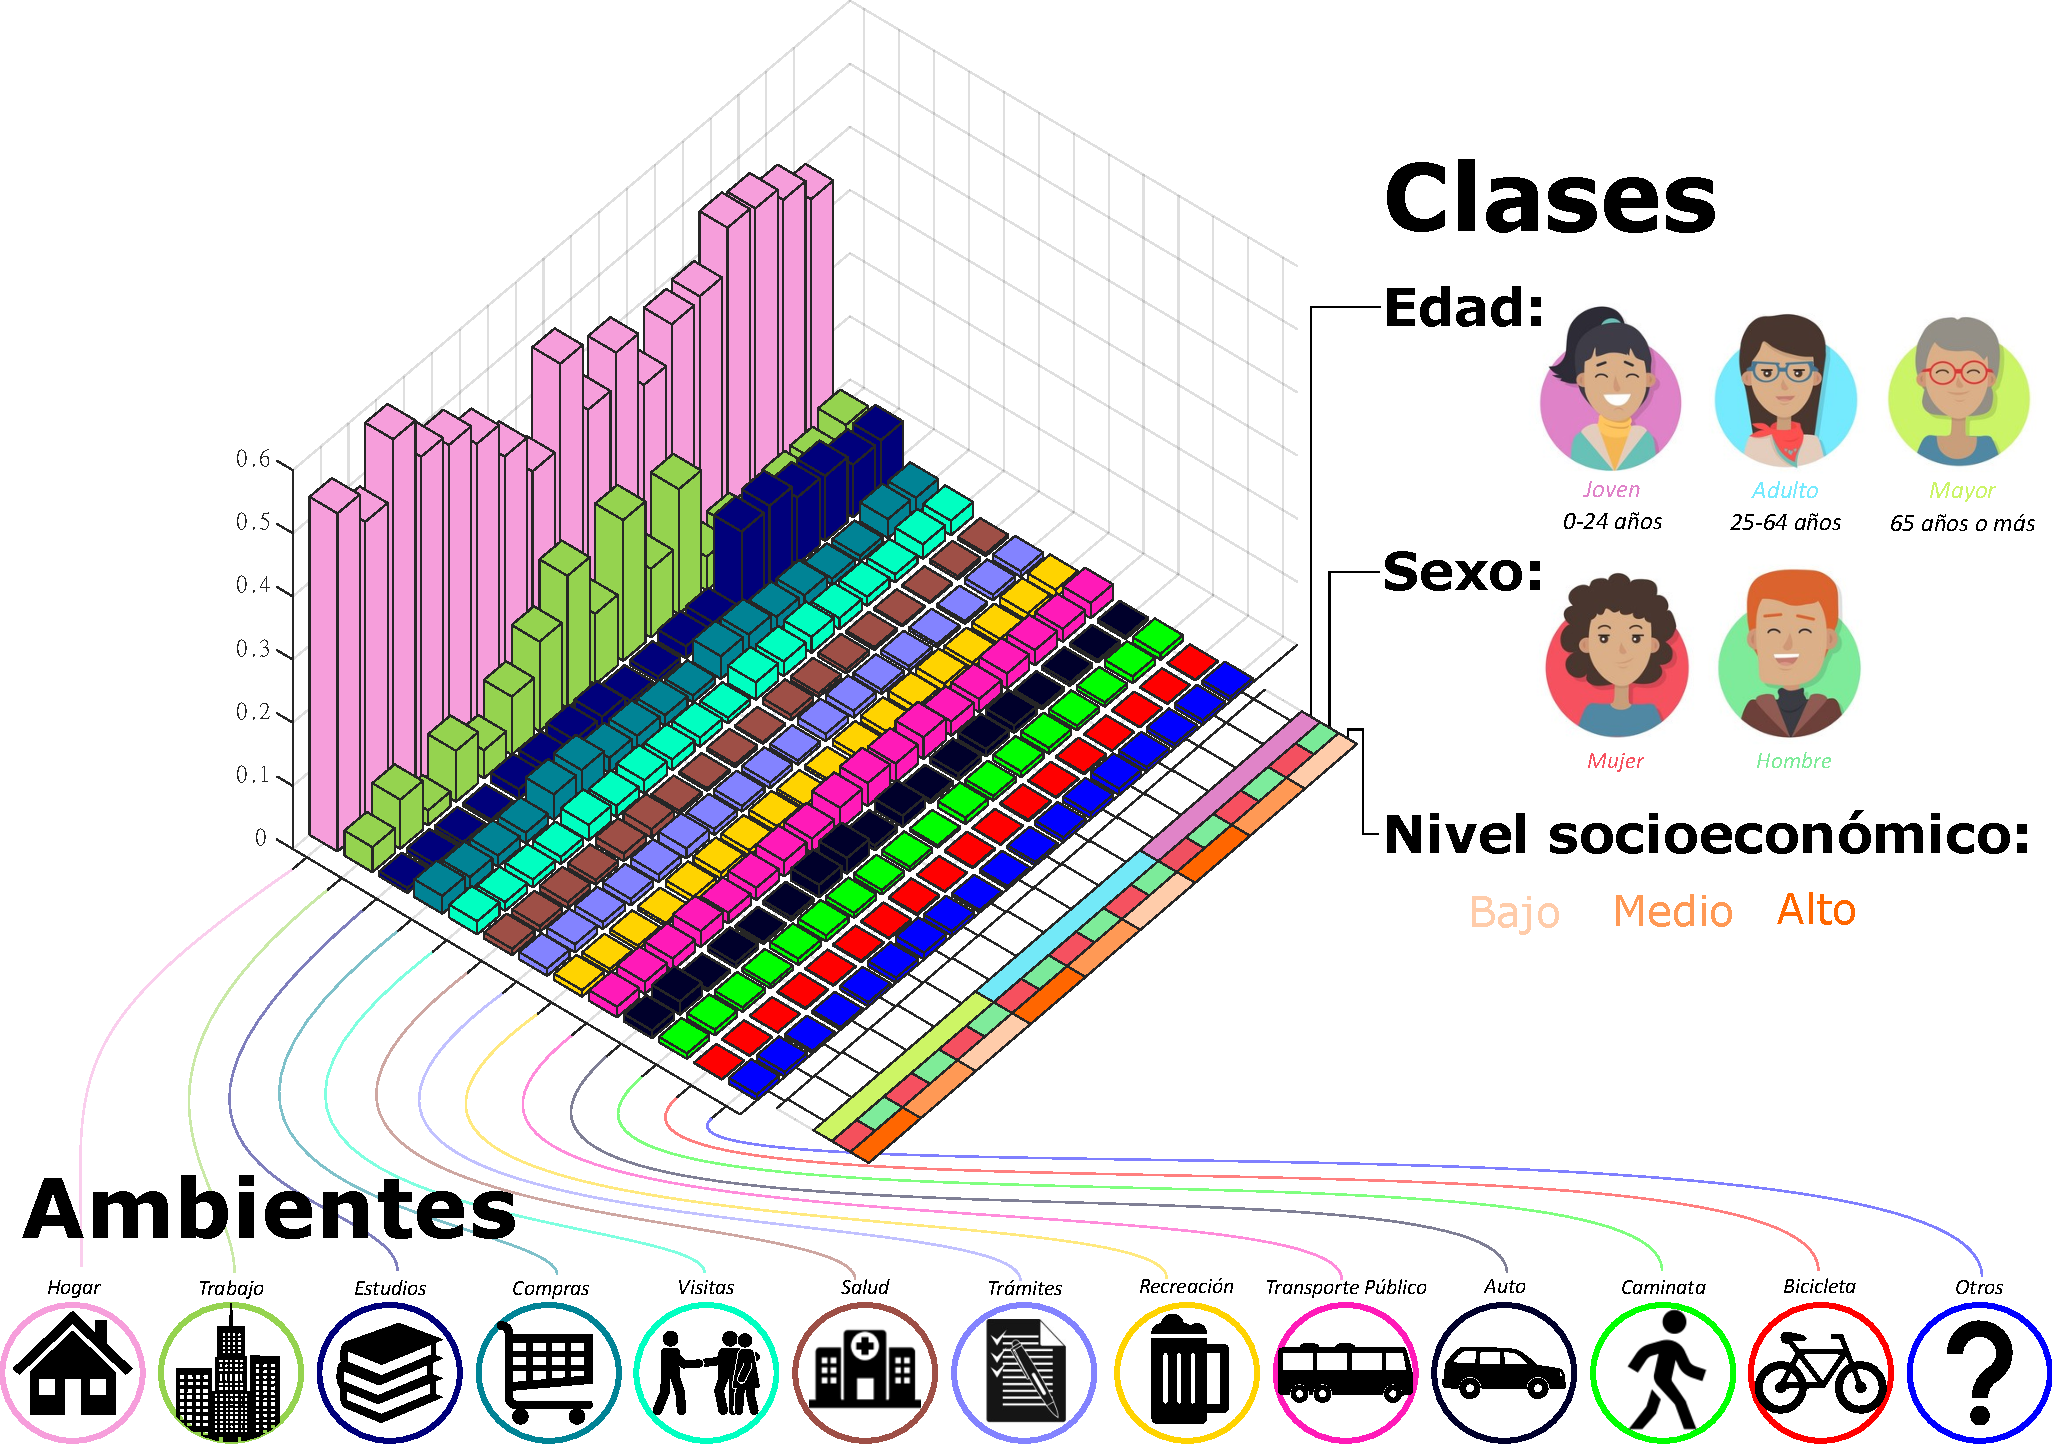
\includegraphics[width=0.99\textwidth]{img/resultados/matrixP/matriz Pambientesyclases.pdf}
\caption[Matriz detallada de tiempos de residencia para Santiago]{Matriz detallada de tiempos de residencia para Santiago. Considera clases basadas en nivel socioeconómico (según ingreso promedio del hogar), edad y sexo. 13 ambientes, basados en los propósitos de viajes de la encuesta. Se restan 7 horas del tiempo en el hogar (tiempo de sueño) y se normalizan las filas para que sumen 1.}
\label{img:Pmatrix-full}
\end{figure}

\subsubsection*{Matriz para las simulaciones}\label{res:matrix-normal-simulaciones}
%\noindent \textbf{Matriz para las simulaciones}

La aplicación del algoritmo tomando en consideración las decisiones tomadas en la sección \ref{subsec:eleccion-clases-ambientes}, específicamente la elección de 5 clases agrupadas por IPS como se detalla en la tabla \ref{table:ips-categ}, y del uso de los ambientes \texttt{hogar} y \texttt{exterior} da lugar a una matriz de tiempos de residencia mucho más sencilla, presentada en la tabla \ref{table:matrix-simulaciones}.

\begin{table}[h!]
\centering
\begin{tabular}{||c c | c c ||} 
 \hline
 \textbf{Clase} & \textbf{Prioridad Social} &  \(P^0_{:,\text{hogar}}\) & \(P^0_{:,\text{exterior}}\)\\[1ex] 
 \hline
 1 & Sin Prioridad  & 0.73  & 0.27 \\ 
 2 & Baja           & 0.76  & 0.24 \\
 3 & Media Baja     & 0.77  & 0.23 \\
 4 & Media Alta     & 0.77  & 0.23 \\
 5 & Alta           & 0.77  & 0.23 \\ 
 \hline
\end{tabular}
\caption[Matriz de tiempos de residencia para las simulaciones.]{Matriz de tiempos de residencia para las simulaciones. La clase sin prioridad corresponde a la más acomodada y la clase con prioridad alta a la más vulnerable.}
\label{table:matrix-simulaciones}
\end{table}

\subsection{Santiago a lo largo del tiempo} \label{res:matrix-pandemia}

Una vez que una matriz \(P^0\) ha sido calculada, se requiere modificar esta matriz a fin de obtener \(P(t)\) que refleje el comportamiento de la población en pandemia.. Estas modificaciones se hacen utilizando los datos de movilidad, siguiendo la metodología presentada en \ref{subsec:variaciones}.

\ref{img:mov-pandemia}
\ref{img:Pmatrix-pandemia-exterior}

\begin{figure}[!h]
\centering
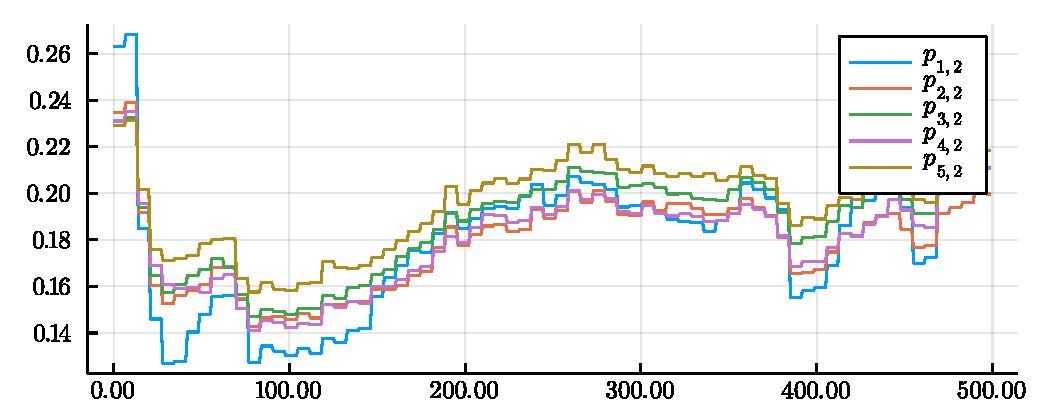
\includegraphics[width=0.99\textwidth]{img/resultados/tiempos-exterior.pdf}
\caption{Fracción de la movilidad en pandemia por grupos, c/r a movilidad normal.}
\label{img:mov-pandemia}
\end{figure}

\begin{figure}[!h]
\centering
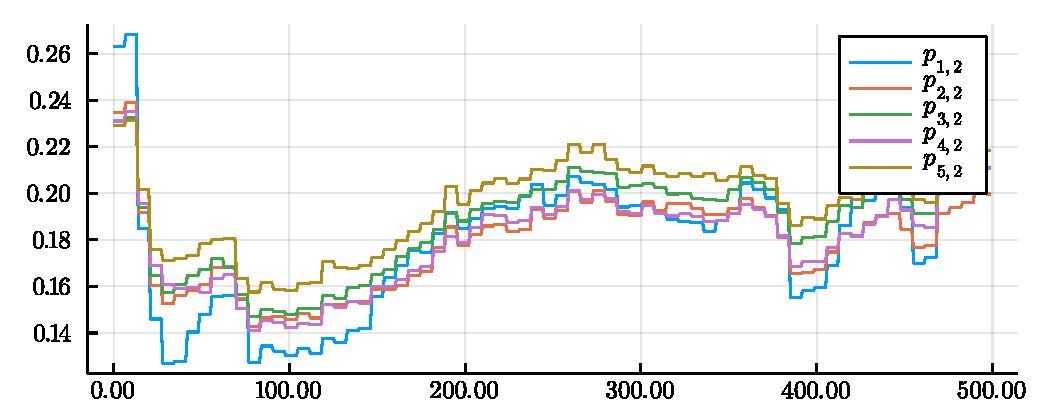
\includegraphics[width=0.99\textwidth]{img/resultados/tiempos-exterior.pdf}
\caption[Tiempo de residencia en \texttt{exterior} para las 5 clases elegidas.]{Tiempo de residencia en \texttt{exterior} para las 5 clases elegidas.}
\label{img:Pmatrix-pandemia-exterior}
\end{figure}